%%\documentclass[12pt,preprint]{aastex}

%% manuscript produces a one-column, double-spaced document:

%\documentclass[manuscript]{aastex}

%% preprint2 produces a double-column, single-spaced document:

 \documentclass[preprint2]{aastex}

%% \documentclass[preprint2,longabstract]{aastex}

\newcommand{\vdag}{(v)^\dagger}
\newcommand{\myemail}{jbyrne@ifa.hawaii.edu}


% ADDING THESE: -JPB
\usepackage{natbib}
\usepackage{amssymb,amsmath}

\shorttitle{3D CMEs Observed with STEREO}
\shortauthors{Byrne et al.}


\begin{document}

\title{3D Reconstructions of Solar Coronal Mass Ejections Observed During the \emph{STEREO} Mission}

\author{J. P. Byrne$^{1}$, et al.} %H. Morgan$^{2,3}$, % P. T. Gallagher$^{4}$, J. M. Refojo$^{5}$, S. R. Habbal$^{1}$}
\affil{$^{1}$Institute for Astronomy, University of Hawai'i, 2680 Woodlawn Drive, Honolulu, HI 96822, USA.\\
	%$^{2}$Sefydliad Mathemateg a Ffiseg, Prifysgol Aberystwyth, Ceredigion, Cymru, SY23 3BZ, UK.\\
	%$^{3}$Coleg Cymraeg Cenedlaethol, Y Llwyfan, Ffordd y Coleg, Caerfyrddin, Cymru, SA31 3EQ, UK.\\
	%$^{4}$School of Physics, Trinity College Dublin, College Green, Dublin 2, Ireland.\\
	%$^{5}$Trinity Centre for High Performance Computing, Trinity College Dublin, College Green, Dublin 2, Ireland.
	}


\begin{abstract}

CMEs are long known to be significant drivers of adverse space weather at Earth, but the physics governing their propagation is not fully understood. The launch of the STEREO mission in 2006 has provided new insight into their motion in the heliosphere, although the mechanisms governing their evolution remain unclear due to difficulties in reconstructing their true 3D structure. Here we use a new elliptical tie-pointing technique to reconstruct a full CME front in 3D, enabling us to quantify an early acceleration profile, non-radial motion, increasing angular width and `pancaking' of the CME front as it propagates from 2\,--\,46~R$_{\odot}$. Beyond 7~R$_{\odot}$, we show that its motion is determined by aerodynamic drag in the solar wind and, using our reconstruction as input for a 3D MHD simulation, we determine an accurate arrival time at the L1 point near Earth.

Analysis of numerous CME observations by \emph{STEREO}, via the 3D elliptical tie-pointing reconstruction technique - building on \citet{2010NatCo...1E..74B}.
\end{abstract}

\keywords{Sun: coronal mass ejections (CMEs) --- Methods: miscellaneous --- Techniques: image processing}


\section{Introduction}

It is predominantly believed that magnetic reconnection is responsible for the destabilisation of magnetic flux ropes on the Sun, which then erupt through the corona into the solar wind to form CMEs \citep{2006GMS...165...43M}. There is much debate as to the specific processes which trigger the eruption of CMEs, and different models exist to explain these \citep{1995ApJ...446..377F, 1996JGR...10127499C, 1999ApJ...510..485A, 2006PhRvL..96y5002K, 2007ApJ...671L..77V}. In the low solar atmosphere, it is postulated that high latitude CMEs undergo deflection since they are often observed at different position angles with respect to their associated source region locations \citep{2009SoPh..259..143X}. It has been suggested that field lines from polar coronal holes may guide high-latitude CMEs towards the equator \citep{angeo-27-4491-2009}, or that the initial magnetic polarity of a flux rope relative to the background magnetic field influences its trajectory \citep{2005A&A...432..331C, 2001SoPh..203..119F}. During this early phase, CMEs are observed to expand outwards from their launch site, though plane-of-sky measurements of their increasing sizes and angular widths are ambiguous in this regard \citep{2009CEAB...33..115G}. This expansion has been modelled as a pressure gradient between the flux rope and the background solar wind \citep{2004ApJ...600.1035R, 1999JGR...104..493O}. At larger distances in their propagation, CMEs are predicted to interact with the solar wind and the interplanetary magnetic field. Studies that compare in-situ CME velocity measurements with initial eruption speeds through the corona show that slow CMEs must be accelerated toward the speed of the solar wind, and fast CMEs decelerated \citep{2009SoPh..256..149M, 2003JGRA..108.1039G}. It has been suggested that this is due to the effects of drag acting on the CME in the solar wind \citep{2006SoPh..233..233T, 2004SoPh..221..135C}. However, the quantification of drag, along with that of both CME expansion and non-radial motion, is currently lacking, due primarily to the limits of observations from single fixed viewpoints with restricted fields-of-view.

Efforts to reconcile 2D plane-of-sky images with the true 3D morphology of CMEs have been underway since they were first observed in the 1970s. The inherent difficulties in this are predominantly due to the single, fixed-position imagers with restricted fields-of-view, as well as the difficulties in observing the optically thin coronal plasma of these dynamic events. Before the launch of STEREO, there was limited ability to infer the 3D CME morphology from the available observations such as SOHO/LASCO. Coronagraphs mainly measure the Thomson scattered light of the free electrons in the coronal plasma, providing white-light images of CMEs against the plane-of-sky that are not trivial to deconvolve,  and the projected 2D nature of these images introduces uncertainties in kinematical and morphological analyses \citep{2007A&A...469..339V}. Some efforts were based upon a pre-assumed geometry of the CME, such as the cylindrical model \citep{2004A&A...422..307C} or the cone model \citep{2005JGRA..11008103X, 2002JGRA..107.1223Z}, whose shapes were simply oriented to best match the 2D observations. Others used either a comparison of multiple events to infer a statistical relationship between plane-of-sky measurements and true CME motion \citep{2005AnGeo..23.1033S, 2005A&A...440..373H}, or a comparison of observations with in-situ data and/or signatures on-disk \citep{2008SoPh..250..347D, 2008JGRA..11301104H}. One prominent method was the use of 3D polarisation analysis of LASCO images \citep{2004Sci...305...66M}, whereby the line-of-sight averaged distance from the plane-of-sky is determined from the brightness ratio of polarised to unpolarised electron scattered emissivity (K-corona). However, this lacks in details such as whether the feature is truly unique along the line-of-sight, and, if so, is it towards or away from the observer with respect to the plane-of-sky. Polarisation analysis itself is only acceptable up to heights of $\sim$\,5~R$_{\odot}$, since beyond this distance the dust-scattered F-corona may no longer be considered unpolarised \citep{1966gtsc.book.....B}. These issues motivated the launch of the STEREO mission to further our understanding of CMEs.


\section{The STEREO Era}

The two near-identical spacecraft of the STEREO mission provide simultaneous observations of CMEs from independent viewpoints to better observe their true morphology. Unfortunately there are limitations on how much 3D information can be extracted from the combined plane-of-sky observations, especially when the object is optically thin and its boundaries ill-defined. In order to determine the morphology of an object in 3D from only two viewpoints, techniques must be applied within the context of an epipolar geometry, as illustrated in Fig.\,? of \citep{2006astro.ph.12649I}. This epipolar coordinate system for considering the 3D space observed from two independent viewpoints is built up as follows. A line is drawn to connect the two observers, called the stereo base line. The two observer locations and any third object point or location in the observing space then define a plane. Numerous object points will define numerous planes that share an intersection with the stereo base line. These are the epipolar planes of Figure~\ref{epipolar}. The plane-of-sky as seen by each observer then intersects the epipolar planes such that they appear as epipolar lines across the image, and will converge on a point along the stereo base line referred to as the epipole of that image. So if a line-of-sight from observer 1 is drawn across an epipolar plane, it will appear as a single point on image 1, but as a complete line across the corresponding epipolar plane in image 2 as seen by observer 2, who is then able to triangulate upon an object in 3D space by the intersecting lines-of-sight. This technique is known as tie-pointing.

\indent The technique of tie-pointing lines-of-sight across epipolar planes is best for resolving a single feature, such as a coronal loop on-disk \citep{2008ApJ...679..827A}. Under the assumption that the same feature may be tracked in coronagraph images many CME studies have also employed tie-pointing techniques \citep{2009SoPh..256...57L, 2009SoPh..259..213S, 2009SoPh..256..183T, 2008SoPh..252..385M, 2009SoPh..259..163W}. However, when measuring the kinematics of the CME front this technique alone doesn't hold true, since it is inevitable that the same part of the curved front cannot be confidently resolved from both viewpoints once the CME has traversed a certain distance in space, nor similarly once the spacecraft have moved beyond a certain angular separation during the mission (see Fig.\,? of \citep{2006astro.ph.12649I}). Furthermore, triangulating CME observations using only the COR images confines the kinematic and morphological analyses to within the 20~R$_{\odot}$ field-of-view. The additional use of the heliospheric imagers allows a study of CMEs out to distances of $\sim$\,1~AU, however (instrumental effects aside) a 3D analysis can only be carried out if the CME propagates along a trajectory between the two spacecraft so that it is observed by both HI instruments. Otherwise, assumptions of its trajectory have to be inferred from either its association with a source region on-disk \citep{2008SoPh..252..373H} or its trajectory through the COR data \citep{2009SoPh..256..149M}, or derived by assuming a constant velocity through the HI fields-of-view \citep{2009GeoRL..3608102D}. Triangulation of CME features using time-stacked intensity slices at fixed latitude, named `J-maps' due to the characteristic propagation signature of a CME, has also been developed \citep{2010SoPh..tmp...49D, 2010ApJ...710L..82L}. This technique is hindered by the same limitation of standard tie-pointing techniques; namely that the curvature of the feature is not considered, and the intersection of sight-lines may not occur upon the surface of the observed feature.

\indent An alternative to tie-pointing is a method called forward modelling which presumes a given shape of the CME and seeks to match it with observational data. \citet{2006ApJ...652..763T} employ a graduated cylindrical shell which is warped to form a flux rope model overlaid on CME images (see Fig.\,? of \citet{2009SoPh..256..111T}). The parameters governing the model's shape and orientation may be changed by the user to fit the model to STEREO-Ahead and Behind data simultaneously and obtain a 3D flux rope characterisation of the CME as it propagates, though this may not always be appropriate \citep{2009ApJ...695L.171J}. \citet{2009SoPh..256..131B} outline a similar forward model which assumes one of three pre-assigned shapes: a hemispherical cap, a flux rope, or a cloud-like model. However, in each of these methods the predetermined shape of the CME model has a spherical cross-section and must adhere to some quasi-similarity (self-invariance) over the sequence of images. So while forward modelling better accounts for the curved nature of the CME being observed, the inherent restrictions of the imposed model still limit the analysis of the true 3D structure and dynamics of the CME as it propagates.



\section{Elliptical Tie-Pointing}
\label{sect:ellipticaltiepointing}

The two near-identical spacecrafts of the STEREO mission provide simultaneous observations of CMEs from independent viewpoints to better determine their true morphology. In order to best characterize the CME structure within the context of an epipolar geometry \citep{2006astro.ph.12649I}, a new method of elliptical tie-pointing was developed by \citet{2010NatCo...1E..74B}. It uses the curvature of the CME as a necessary third constraint on the 3D reconstruction from the two STEREO viewpoints. The technique works by first performing an ellipse characterization of the CME in the SECCHI images\footnote{Movie of SECCHI data:~tinyurl.com/secchi20081212} (left panel of Fig.\,\ref{3Delliptical}). An epipolar plane will intersect the CME in two locations (i.e., front and back of the ellipse), as modeled by \citet{2004GeoRL..3121802P}. Therefore two lines-of-sight that enclose the CME in each image, may be drawn across the epipolar plane until they intersect in 3D space. This results in a quadrilateral bounding shape, into which an ellipse of maximal area and minimal eccentricity is inscribed tangent to each line-of-sight \citep{2005AJMAA..2.1H}. This localizes the position of the CME within the epipolar plane (Fig.\,\ref{3Delliptical}a). Repeating this process for all epipolar planes in which the CME structure resides, allows a 3D localization of the entire CME as constrained by its measured curvature on each plane-of-sky (Fig.\,\ref{3Delliptical}b). This is then repeated for every frame in the observations to build a reconstruction of the CME front through time\footnote{Movie of 3D reconstruction:~tinyurl.com/3dcme20081212} (Fig.\,\ref{3Delliptical}c). Resolving the 3D information of the CME in this unique manner is vital for studying the true dynamics of its motion and evolution through space, as demonstrated by \citet{2010NatCo...1E..74B} in determining the acceleration, drag, deflection and expansion of the Earth-directed CME on 12~Dec.~2008 (reproduced in Fig.\,\ref{kins20081212}).


In the epipolar geometry outlined above, 3D information may be gleaned from two independent viewpoints of a feature using tie-pointing techniques to triangulate lines-of-sight in space. However, when the object is known to be a curved surface, sight-lines will be tangent to it and not necessarily intersect upon it. Consequently CMEs cannot be reconstructed by tie-pointing alone, but rather their localisation may be constrained by intersecting sight-lines tangent to the leading edges of a CME \citep{2004GeoRL..3121802P, 2009SoPh..256..167D}. Following the multiscale edge detection and ellipse characterisation outlined in Chapter~\ref{chapter:multiscale}, it is possible to extract the intersection of a given epipolar plane through the ellipse fits of both the STEREO-Ahead and Behind images. This defines a quadrilateral in 3D space that localises the ellipse characterisation of the CME front in that plane.

Inscribing an ellipse within the quadrilateral such that it is tangent to all four sides (detailed below) provides a slice through the CME that matches the observations from each spacecraft (Fig.\,? of \citet{2010NatCo...1E..74B}). A full reconstruction is achieved by stacking ellipses from numerous epipolar slices. Since the positions and curvatures of these inscribed ellipses are constrained by the characterised curvature of the CME front in the stereoscopic image pair, the modelled CME front is considered an optimum reconstruction of the true CME front. This is repeated for every frame of the eruption to build the reconstruction as a function of time and view the changes to the CME front as it propagates in 3D.

Following \citet{2002SWJPAM..1.6H, 2005AJMAA..2.1H}, we inscribe an ellipse within a quadrilateral using the following steps (see Figure~\ref{ellipseinscribed}):

\begin{figure}[!t]
\centerline{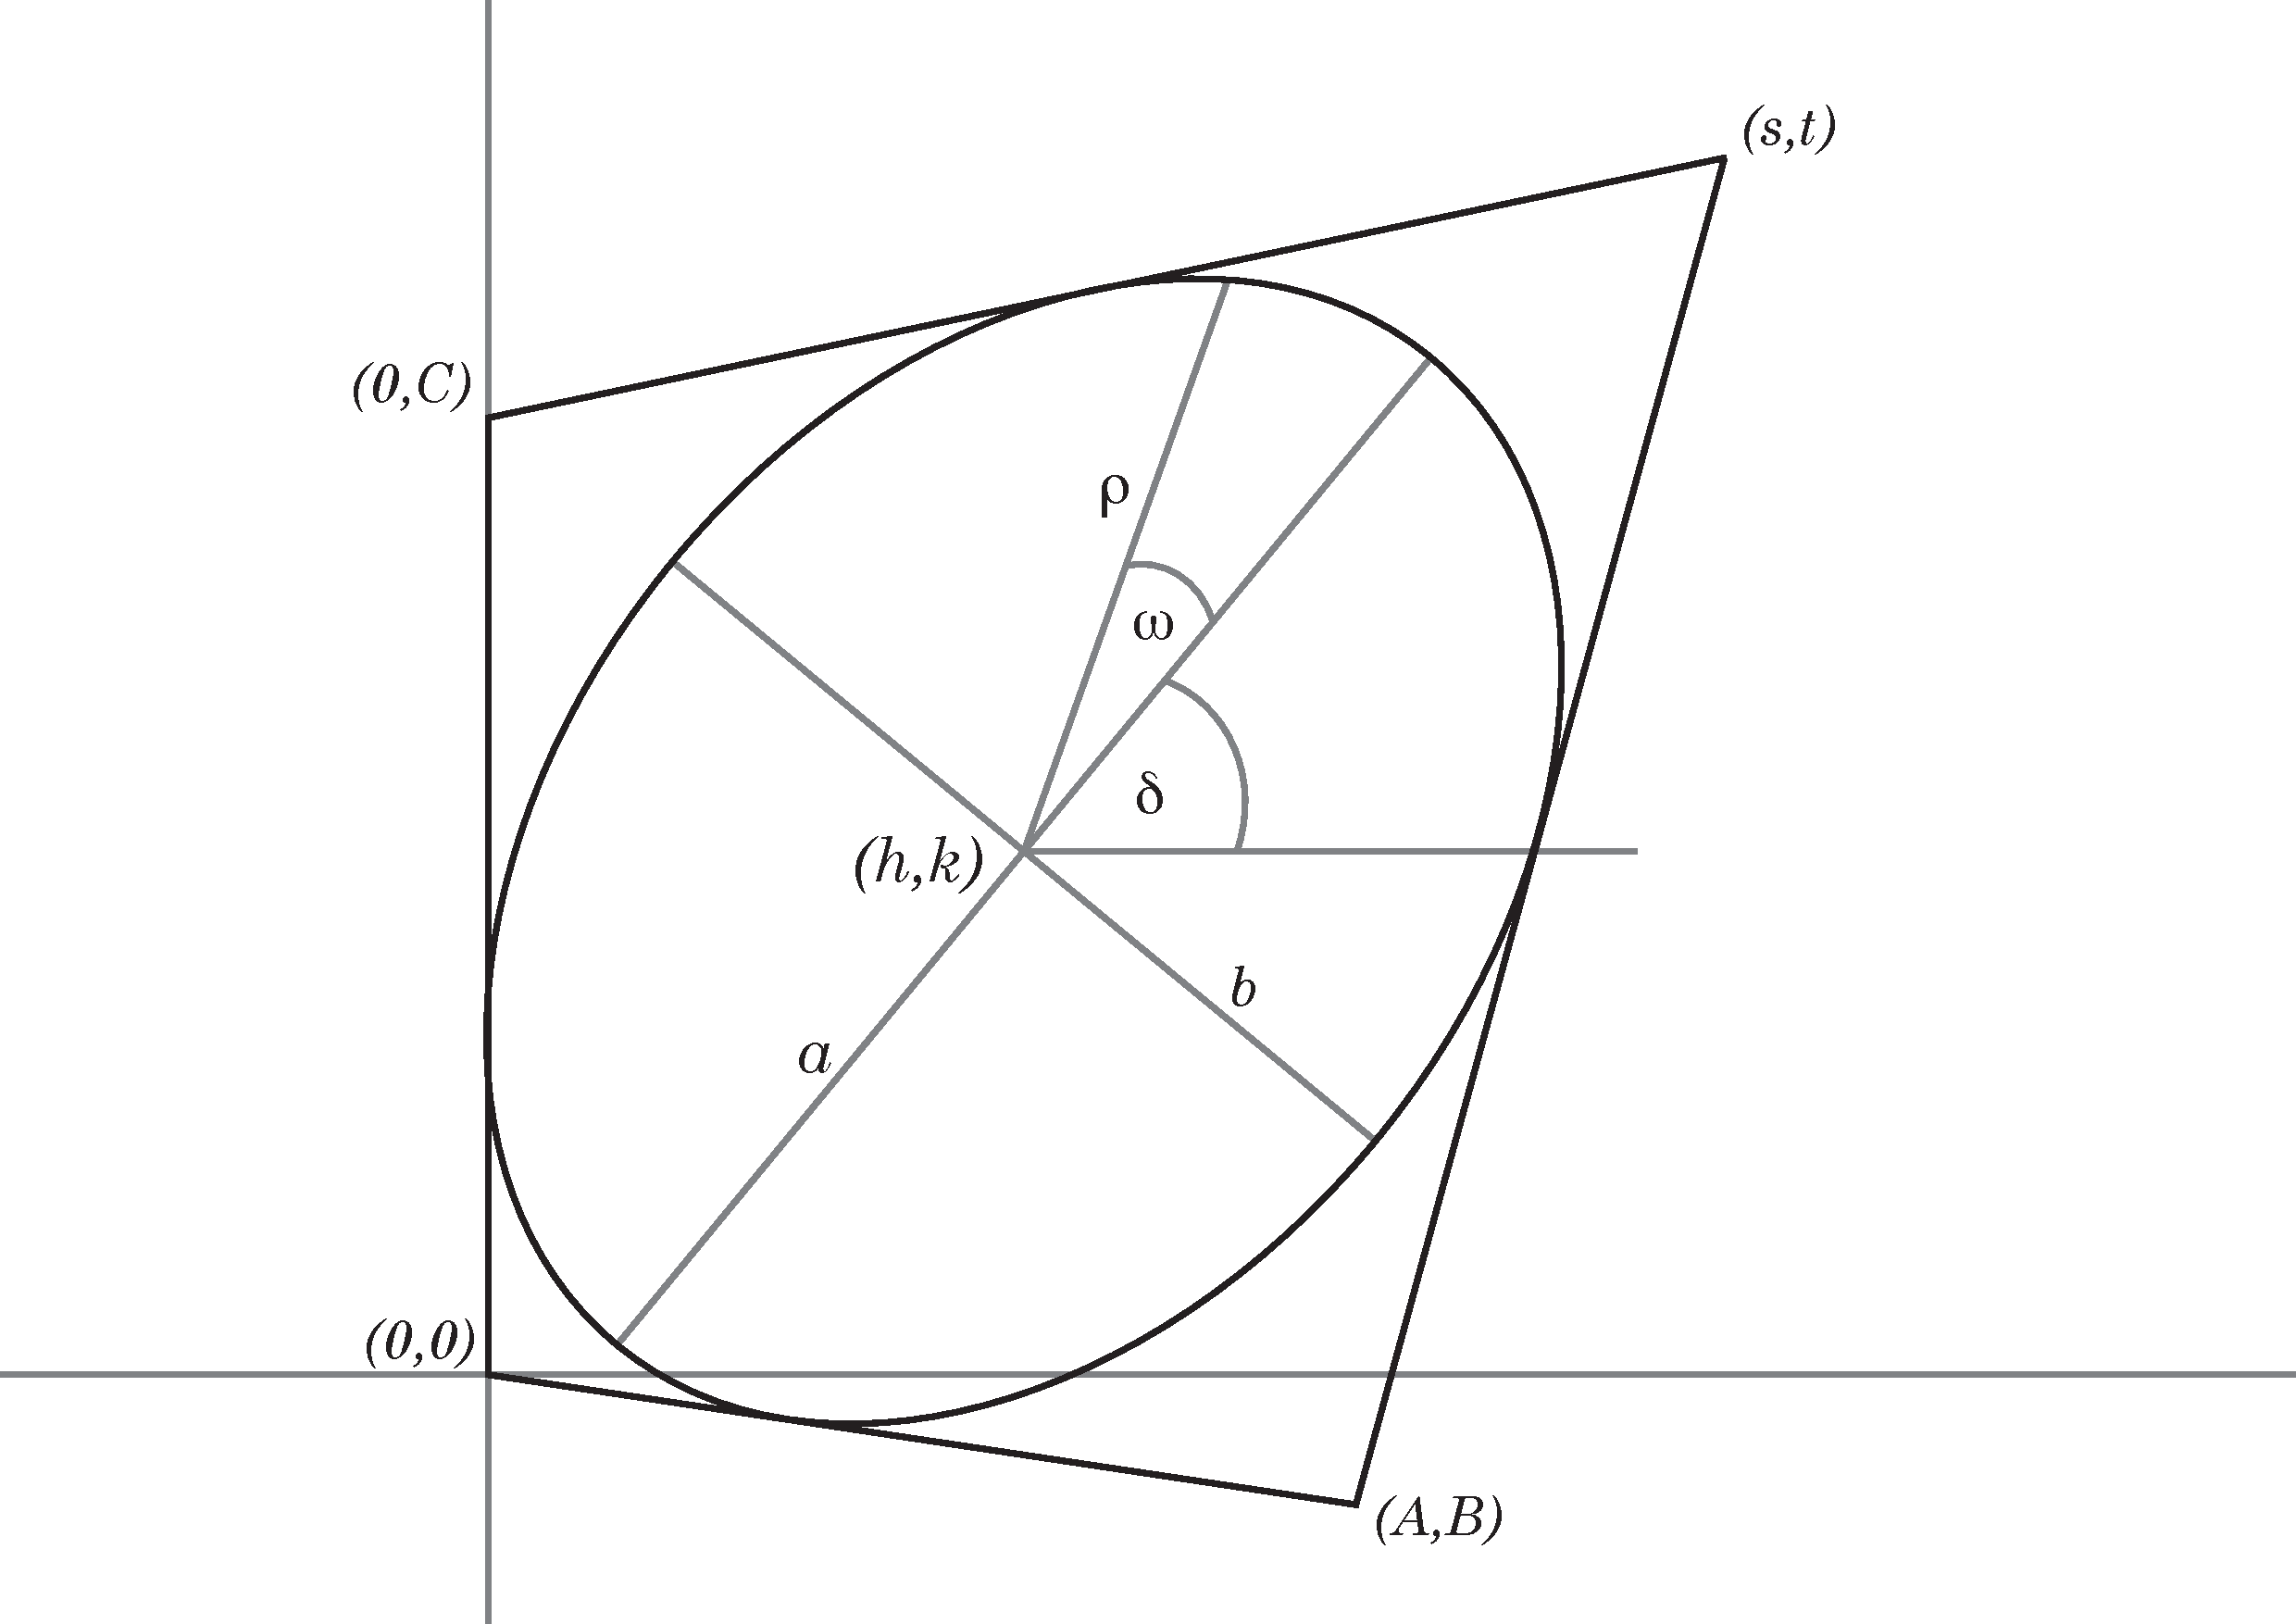
\includegraphics[width=\linewidth, scale=0.25, clip=true, trim=150 0 200 0]{images/ellipseinscribed.pdf}}
\caption{An ellipse inscribed within a convex quadrilateral. An isometry of the plane is applied such that the quadrilateral has vertices $(0,0)$, $(A,B)$, $(0,C)$, $(s,t)$. The ellipse has centre $(h,k)$, semimajor axis $a$, semiminor axis $b$, tilt angle $\delta$, and is tangent to each side of the quadrilateral.}
\label{ellipseinscribed}
\end{figure}

\begin{enumerate}

\item Apply an isometry to the plane such that the quadrilateral has vertices $(0,0)$, $(A,B)$, $(0,C)$, $(s,t)$, where $A>0$, $C>0$, $s>0$ and $t>B$. (Note, in the case of an affine transformation we set $A=1$, $B=0$ and $C=1$, with $s$ and $t$ variable.)

\item Set the ellipse centre point $(h, k)$ by fixing $h$ somewhere along the open line segment connecting the midpoints of the diagonals of the quadrilateral and hence determine $k$ from the equation of a line, for example:
\begin{eqnarray}
h\,=\,\frac{1}{2}\left(\frac{s}{2}+\frac{A}{2}\right) \\
k\,=\,\left(h-\frac{s}{2}\right)\left(\frac{t-B-C}{s-A}\right) + \frac{t}{2}
\end{eqnarray}

\item To solve for the ellipse tangent to the four sides of the quadrilateral, we can solve for the ellipse tangent to the three sides of a triangle whose vertices are the complex points
\begin{eqnarray}
z_{1} = 0, \quad
z_{2} = A+Bi, \quad
z_{3} = -\frac{At-Bs}{s-A}i
\end{eqnarray}
and the two ellipse foci  are then the zeroes of the equation
\begin{eqnarray}
p_{h}(z) \;=\; \left(s-A\right)z^{2}-2\left(s-A\right)\left(h-ik\right)z-\left(B-iA\right)\left(s-2h\right)C
\end{eqnarray}
whose discriminant can be denoted by $r(h)=r_{1}(h)+ir_{2}(h)$ where
\begin{align} \nonumber
r_1 \;=\; &4 \left(\left(s-A\right)^{2}-\left(t-B-C\right)^{2}\right)\left(\frac{h-A}{2}\right)^{2} \\ \nonumber
 &+4 \left(s-A\right)\left(A\left(s-A\right)+B\left(B-t\right)+C\left(C-t\right)\right)\left(\frac{h-A}{2}\right) \\
 &+ \left(s-A\right)^{2}\left(A^{2}-\left(C-B\right)^{2}\right) \\ \nonumber
r_2 \;=\; &8\left(t-B-C\right)\left(s-A\right)\left(\frac{h-A}{2}\right)^{2} \\ \nonumber
&+ 4\left(s-A\right)\left(At+Cs+Bs-2AB\right)\left(\frac{h-A}{2}\right) \\
&+ 2A\left(s-A\right)^{2}\left(B-C\right)
\end{align}
Thus we need to determine the quartic polynomial $u(h)=|r(h)|^{2}={r_1(h)}^{2}+{r_2(h)}^{2}$ and we can then solve for the ellipse semimajor axis, $a$, and semiminor axis, $b$, from the equations
\begin{eqnarray}
a^{2}-b^{2} \;=\; \sqrt{ \frac{1}{\left(16\left(s-A\right)^{4}\right)}u(h)} 
\end{eqnarray}
\begin{eqnarray}
a^{2}b^{2} \;=\; \frac{1}{4}\left(\frac{C}{\left(s-A\right)^{2}}\right)\left(2\left(Bs-A\left(t-C\right)\right)h - ACs\right)\left(2h-A\right)\left(2h-s\right) 
\end{eqnarray}
by parameterising $R=a^{2}-b^{2}$ and $W=a^{2}b^{2}$ to obtain
\begin{eqnarray}
a \;=\; \sqrt{ \frac{1}{2}\left(\sqrt{R^{2}+4W}+R\right)}, \\
b \;=\; \sqrt{ \frac{1}{2}\left(\sqrt{R^{2}+4W}-R\right)}
\end{eqnarray}
\item Knowing the axes we can generate the ellipse and float its tilt angle $\delta$ until it sits tangent to each side of the quadrilateral, using the inclined ellipse equation~(\ref{eqn:inclinedellipse}) introduced in Section~\ref{sect:characterisation}.
%\begin{eqnarray}
%\rho^{2} \;=\; \frac{a^{2}b^{2}}{\left(\frac{a^{2}+b^{2}}{2}\right)-\left(\frac{a^{2}-b^{2}}{2}\right)\cos\left(2\omega'-2\delta\right)}
%\end{eqnarray}
%where $\omega'=\omega+\delta$ and $\omega$ is the angle from the semimajor axis to a radial line $\rho$ on the ellipse.
\end{enumerate}
\noindent

\section{3D Reconstruction Model \& Error Quantification}


\begin{figure}[ht]
\includegraphics[scale=0.2, trim=0 0 0 0, clip=true]{images/fluxropemodel.jpg}
\caption{Model flux-rope CME}
\label{fluxropemodel}
\end{figure}

\begin{figure}[!ht]
\centering{\includegraphics[width=\linewidth]{images/dets_splice.pdf}}
\caption{Synthetic observations of a model CME flux-rope observed by the STEREO/COR2 coronagraphs, at a spacecraft separation of $90^{\circ}$. The CME is Earth-directed, shown here with an orientation of $0^{\circ}$, i.e., the flux-rope axis is parallel to the ecliptic. The automated CORIMP CME detection algorithm was applied, highlighting the CME structure and outer front. A 3D reconstruction is then performed using the elliptical tie-pointing technique, in order to test the fidelity of the methods and quantify the uncertainty on any resulting measurements.}
\label{dets_splice}
\end{figure}

\begin{figure*}
\centering{\includegraphics[scale=0.25, trim=0 0 0 0]{images/model_recon_panels.pdf}}
\caption{The 3D CME front reconstruction (in black) of a model CME flux-rope (in blue) via the elliptical tie-pointing methodology from the observations of STEREO-A (in red) and STEREO-B (in green). The Sun is shown at location (0,0,0) in a Heliocentric Earth Equatorial coordinate system (HEEQ). The top panels show a model flux-rope at 0$^{\circ}$~orientation (parallel to the ecliptic), while the bottom panels show it at 90$^{\circ}$~orientation (perpendicular to the ecliptic); with a general view, side view, and top view of each case.}
\label{3d_panels}
\end{figure*}


In order to test the possible uncertainties to be attributed to 3D reconstructions via the elliptical tie-pointing technique, a model flux-rope CME was developed (extended from \citealt{2012ApJ...752..144M}) so that synthetic coronagraph observations may be generated for a  CME observed at any STEREO spacecraft separation, propagating with any given trajectory, orientation and brightness. These model observations may be analyzed with the CORIMP CME detection and tracking routines (as in Fig.\,\ref{dets_splice}), and the resulting CME fronts fitted with ellipses to characterize their motion across each plane-of-sky. A 3D reconstruction may then be generated and directly compared with the model itself to inspect the fidelity of the technique. \emph{Note that this is simply to provide a quantification of the possible error involved in the 3D reconstruction technique itself, as its efficiency will be affected mainly by different spacecraft separations, and to a lesser extent by different CME orientations and trajectories.} Any resulting offset that would affect the accuracy of measurements on the CME morphology (e.g., the heights of the CME front and resulting kinematic profiles) may therefore be quantified. This provides a measure of the uncertainty involved when the reconstruction is performed on real data.

For example, a model CME was generated to match the event scenario of the previously studied 12~Dec.~2008 Earth-directed CME when the spacecrafts were almost in perfect quadrature. The 3D reconstruction of the model at two instances of orientation is overlaid on the model itself in Fig.\,\ref{3d_panels}: the top panels correspond to a flux-rope axis parallel to the ecliptic (orientation angle $0^{\circ}$), and the bottom panels correspond to a flux-rope axis perpendicular to the ecliptic (orientation angle $90^{\circ}$); with a general view, side view, and top view displayed for each case. The model is in blue, with the reconstructed CME front overlaid in black, from the observations of STEREO-A in red, and STEREO-B in green. An initial inspection reveals the case of $0^{\circ}$~orientation proves more accurate with negligible offsets in the front height measurements, while the $90^{\circ}$~orientation can have up to $\sim$10\% offset at its apex. Inspection of the SECCHI and LASCO observations of the 12~Dec.~2008 CME can be used to constrain the model, implying a more symmetrical flux-rope would be appropriate, with an orientation no more extreme than $\sim$30$^{\circ}$. Using the LASCO characterizations of the event to help constrain the 3D reconstruction (as described in \S\,3.2 above) will help determine the true spatial extent and possible orientation of the CME in order to best consider a model for testing the uncertainties in the reconstruction technique for such a scenario. Quantifying these uncertainties will lead to a better error treatment of the true 3D kinematics of CME reconstructions, allowing a correction to be applied to any offset in the height-time measurements where appropriate, or at least a justified uncertainty interval be assigned to any measurements derived from the 3D reconstruction.


\section{Observations}

\subsection{SOHO Observations as a `Third-Eye'}


The SOHO spacecraft offers a `third-eye' to STEREO observations of the Sun and CMEs, with the LASCO coronagraphs having fields-of-view of 2\,--\,6\,R$_{\odot}$ (C2) and 4\,--\,30\,R$_{\odot}$ (C3). This allows an overlap with the SECCHI instruments that cover 1.3\,--\,4\,R$_{\odot}$ (COR1) and 2\,--\,15\,R$_{\odot}$ (COR2), therefore observing most events that STEREO observes, but from a fixed location about L1. As the STEREO spacecrafts separate throughout the mission lifetime, the efficiency of a triangulation technique changes, being most effective at times when the spacecrafts are close to quadrature (90$^{\circ}$ separation from each other). When they moved away from their initial quadrature positioning on the near-side of the Sun in 2008/9, they began observing in near-quadrature with the SOHO spacecraft over the course of 2010/11. This represents a phase in the mission when the combination of SOHO and STEREO observations could be used to overcome the limitations of the reconstruction technique when STEREO are in opposition ($\sim$180$^{\circ}$ separation).

To this end, the elliptical tie-pointing methodology has been extended for combining LASCO coronagraph observations with those of the SECCHI coronagraphs, as demonstrated in Fig.\,4 of \citealt{2013NatPh...9..811C} for a CME on 22~Sept.~2011 (with an associated shock). This CME appeared as a halo towards the STEREO-B spacecraft, off the east limb in the LASCO observations, when STEREO-B was at a separation of 96.5$^{\circ}$ from Earth and SOHO (Fig.\,\ref{SOHO+STEREO_figure}a). The ellipse characterization of the flux-rope CME discernible in the C2 images provides a constraint on the extent of the CME in the fainter signal of the COR1 images. This is demonstrated by the red points on the north and south flanks of the C2 ellipse characterization in Fig.\,\ref{SOHO+STEREO_figure}b, that correspond to the red lines-of-sight across the COR1 image in Fig.\,\ref{SOHO+STEREO_figure}c. Ultimately a 3D reconstruction of the CME was realized via this new extension of the elliptical tie-pointing technique to combine SOHO with STEREO observations, as shown in Fig.\,\ref{SOHO+STEREO_figure}d.

Since the cadence times of the SOHO and STEREO coronagraphs are generally offset from each other by varying amounts (except for some serendipitous timings such as the example in Fig.\,\ref{SOHO+STEREO_figure}), a method of ellipse interpolation will be used to determine plane-of-sky information in between LASCO frames, at times corresponding to the SECCHI cadence. This is demonstrated in Fig.\,\ref{ellipse_params} for a CME observed on 22~May~2013. The leading edge of the CME is characterized by the ellipses shown in the left of Fig.\,\ref{ellipse_params}, over-plotted on the first observation of the CME in LASCO/C2 at 09:12\,UT. The right plot of Fig.\,\ref{ellipse_params} shows the ellipse parameters of center coordinates $x$ and $y$, the semi-axes lengths, and the tilt angle of the ellipse. The time evolution of each parameter is fit with a cubic spline such that an interpolated ellipse may be generated at any given time-stamp, demonstrated here for the corresponding COR1 observation of the event at 10:08\,UT (over-plotted in green on the C2 image). Thus the cadence offset can be overcome and a 3D reconstruction of the events observed by SOHO and STEREO may be generated in the same manner as the example of Fig.\,\ref{SOHO+STEREO_figure}. This therefore makes it possible to perform 3D reconstructions of CMEs observed by any two of the three SOHO and STEREO-Ahead or Behind spacecrafts. 


\begin{figure*}[ht]
\centering{\includegraphics[width=\linewidth, scale=0.25, trim=0 0 0 230]{images/ellipse_params.pdf}}
\caption{The ellipse characterizations of a CME observed by SOHO/LASCO on 22 May 2013, first seen in C2 at 09:12:08\,UT. The centre-point coordinates, axes lengths, and tilt angles of the white ellipse characterizations of the CME front are plotted against time on the right. The vertical dashed line indicates the time-stamp of a STEREO/COR1 observation of this event at 10:08:15\,UT. The spline-interpolated ellipse parameters are used to generate a corresponding ellipse at that time-stamp, plotted in green on the C2 image. This overcomes the cadence offset of the SOHO and STEREO coronagraphs, enabling a 3D reconstruction of the event via the elliptical tie-pointing technique on the combined observations.}
\label{ellipse_params}
\end{figure*}


\subsection{3D CME Dynamics: Revisiting the 12~Dec.~2008 event}

\begin{figure}[ht]
\centering{\includegraphics[scale=0.37, trim=20 100 0 100]{images/12dec2008kins.pdf}}
\caption{The kinematics of the prominence and 3D reconstructed CME front of the 12~Dec.~2008. The prominence is observed as the inner material of the CME, with both undergoing acceleration from $\sim$\,06:00\,--\,07:00\,UT, peaking at $\sim$\,40\,m\,s$^{-2}$ and $\sim$\,94\,m\,s$^{-2}$ respectively, before reducing to scatter about 0. Measurment uncertainties are indicated by one standard deviation error bars.}
\label{12dec2008kins}
\end{figure}

\begin{figure*}[!hp]
\centering{\includegraphics[scale=0.7, trim=0 60 0 100]{images/kins_inspect.png}}
\caption{3D CME front reconstruction heights (top), velocities (middle) and accelerations (bottom) derived from quadratic fits to the height-time profiles measured along every latitude and longitude angle of propagation. The median, interquartile ranges, and upper/lower fences of the velocity and acceleration plots are shown as the solid, dashed, and dotted lines respectively.}
\label{kins_inspect}
\end{figure*}

Using these novel 3D reconstruction techniques in tandem with the highly accurate and robust CORIMP techniques, enables improved determinations of the 3D dynamics of CMEs. Specifically in the case of CME kinematics, a recent investigation by \citet{2013A&A...557A..96B} highlights improved methods for determining the velocity and acceleration profiles of CMEs, and quantifying the uncertainties in their derived values. The spread of height-time measurements across the CME front provide a measure of the bulk kinematics, with insight to the early acceleration onset that signifies the main energy release. The rigor that improved methods for determining CME kinematics can provide, must now be extended to the 3D reconstructions of CMEs as they erupt and propagate away from their source regions on the Sun, in order to overcome plane-of-sky effects and determine the true dynamics of their motion.

One such example of the breadth of information obtainable from rigorous kinematic studies is shown in Fig.\,\ref{kins_inspect}, for the 3D CME front reconstruction of the 12~Dec.~2008 event from \citealt{2010NatCo...1E..74B}. In that particular study, a true height-time profile of the CME was measured from the apex of the reconstructed CME front along the Sun-Earth line (see Fig.\,\ref{12dec2008kins}), to be linked with the in-situ detections of the WIND spacecraft at L1. However, the 3D reconstruction may be inspected in much greater detail: for example, by taking the height-time measurements at every latitude and longitude angle of propagation. This can reveal changes to the CME morphology as it can undergo deflection and/or asymmetric expansion as a result of the forces driving its propagation. The plots of Fig.\,\ref{kins_inspect} show the resulting distributions of heights, velocities and accelerations ($z$-axis), against time ($x$-axis), for every longitude ($y$-axis) and latitude (colorbar) of the CME propagation (relative to the Sun-Earth line at 0$^{\circ}$ latitude and 0$^{\circ}$ longitude). The velocities and accelerations shown here are derived from quadratic fits to the height-time profiles of the CME front. Note that some points of varying color are obscured by overlapping plot symbols. The solid, dashed, and dotted lines on the back surfaces of the velocity and acceleration plots indicate the bulk medians, interquartile ranges, and upper/lower fences on the distribution of derived measurements. These reveal the trends of increasing bulk velocity of the CME towards a value of $\sim$600$\,km\,s^{-1}$, from an initially peaked acceleration of $\sim$20$\,m\,s^{-2}$ leveling off to $\sim$5$\,m\,s^{-2}$.

It may be further noted that in the height-time-longitude plot of Fig.\,\ref{kins_inspect}\,(\emph{top}), the color gradient representing the latitudes at which the measurements were made, transition from the redder end to the bluer end in a somewhat diagonal fashion up the datapoints. This is an indication of the deflected motion of the CME, as it moves in a non-radial trajectory from its source region observed on the disk at a latitude of $\sim$54$^{\circ}$\,N to propagate along the plane of the ecliptic towards Earth (see Fig.\,3b of \citealt{2010NatCo...1E..74B}).


\acknowledgments

This work is supported by SHINE grant 0962716 and NASA grant NNX08AJ07G to the Institute for Astronomy. %The \emph{SOHO}/LASCO data used here are produced by a consortium of the Naval Research Laboratory (USA), Max-Planck-Institut fuer Aeronomie (Germany), Laboratoire d'Astronomie (France), and the University of Birmingham (UK). SOHO is a project of international cooperation between ESA and NASA. \emph{SDO} data supplied courtesy of the NASA/\emph{SDO} consortia.
The \emph{STEREO}/SECCHI project is an international consortium of the Naval Research Laboratory (USA), Lockheed Martin Solar and Astrophysics Lab (USA), NASA Goddard Space Flight Center (USA), Rutherford Appleton Laboratory (UK), University of Birmingham (UK), Max-Planck-Institut f\"{u}r Sonnen-systemforschung (Germany), Centre Spatial de Liege (Belgium), Institut d'Optique Th\'{e}orique et Appliqu\'{e}e (France), and Institut d'Astrophysique Spatiale (France).
%\appendix

%\section{Appendix material}

%For completeness, here is one last equation.
%\begin{equation}
%e = mc^2
%\end{equation}

\bibliographystyle{apj.bst}
\bibliography{references.bib}  


\end{document}